\subsection{Color Preservation}
Another feature we implemented in our video style transfer is color preservation. One limitation with normal style transfer is the fact that it transfers the style from one particular painting or picture. That means both the style and the color of the style image is transferred to our generated image. This can work fine in some instances, but in some cases we want to transfer only the styling and keep the original color of our image. For example if we want to transfer the painting style from a famous painter, we do not necessarily also want to transfer the color of that particular painting This is the purpose of implementing color preservation.\newline\newline
Our implementation is based on the "Luminance-only transfer" approach described in the paper of Gatys et al. \cite{Gatys:2}. To implement color preservation we just need to add a few components. After we first load our original photo, we save the color profile of the photo. This is saved as an YUV file, because unlike RGB, YUV has an attribute to save the luminosity of the picture. After this we continue the styling process and training until we have the completed stylized picture. Then finally we transfer the color profile and luminosity of the original picture to the stylized picture. Now we have successfully transferred the styling to our picture while preserving the colors from our original photo.\newline
e.g styling an image with van Gogh's Starry night:\newline
\begin{figure}[!ht]
\begin{center}
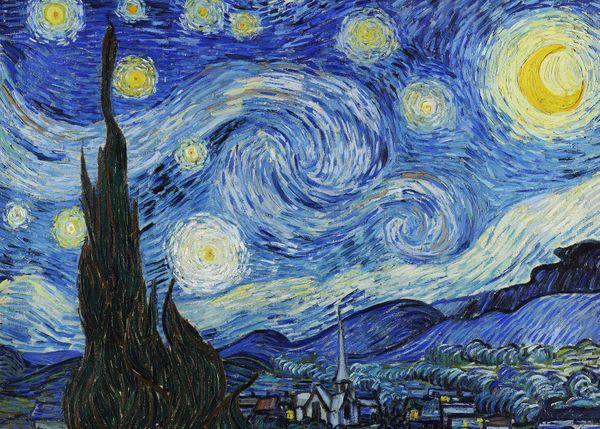
\includegraphics[width=0.4\textwidth]{report/Method/images/style_starry_night.jpg}
\label{fig:starry night}\newline


\includegraphics[width=0.32\textwidth]{report/Method/images/original_cat.png}
\label{original cat}
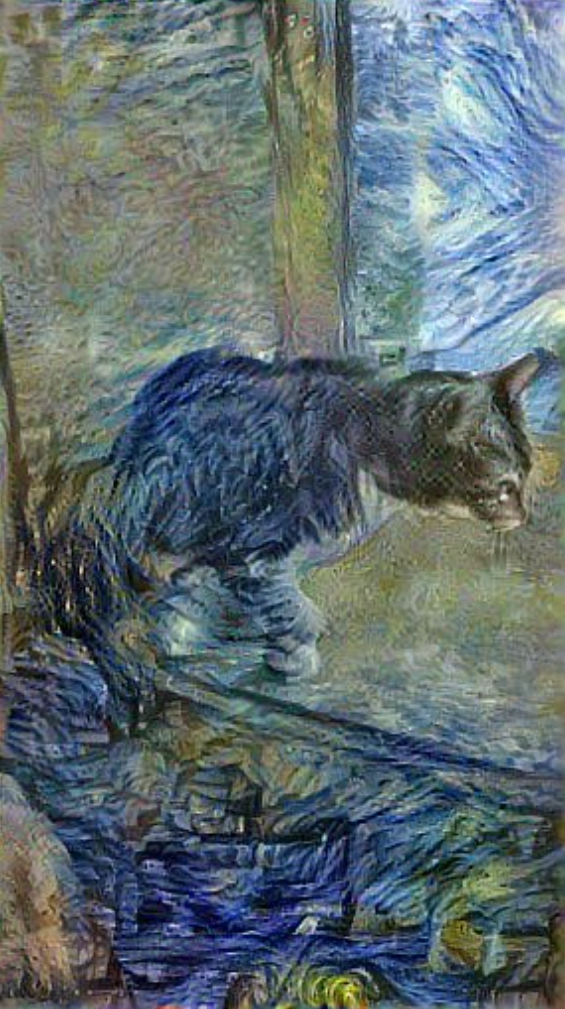
\includegraphics[width=0.32\textwidth]{report/Method/images/styled_cat.png}
\label{styled cat}
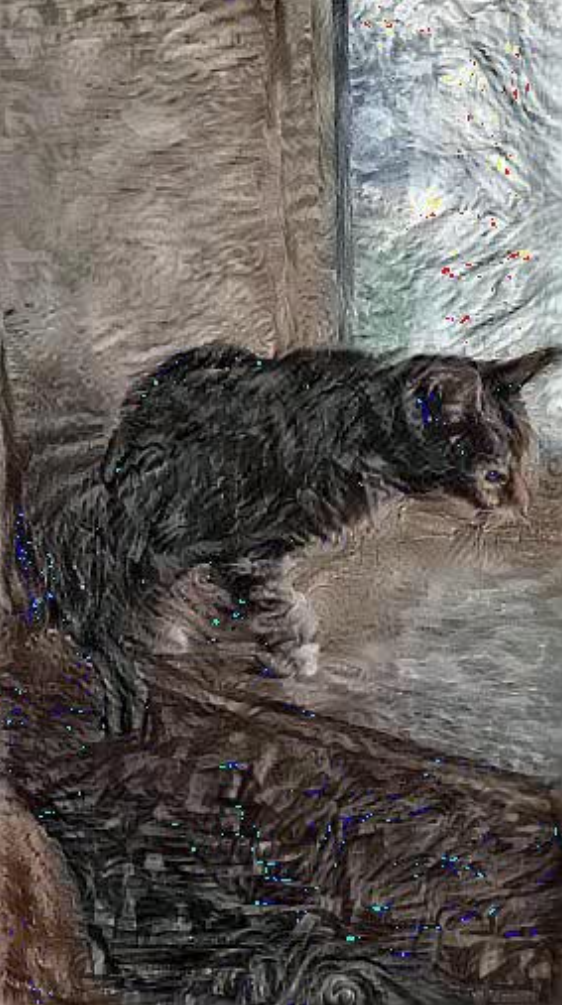
\includegraphics[width=0.32\textwidth]{report/Method/images/color_preserved.png}
\label{color preserved cat}
\caption{To the left is the original picture, middle is the styled picture, right side is the styled picture with color preservation.}
\end{center}
\end{figure}
\newpage



